\subsection*{试题背景}

顿顿在学习了数字图像处理后,想要对手上的一副灰度图像进行降噪处理。不过该图像仅在较暗区域有很多噪点,如果贸然对全图进行降噪,会在抹去噪点的同时也模糊了原有图像。因此顿顿打算先使用{\heiti{邻域均值}}来判断一个像素是否处于{\heiti{较暗区域}},然后仅对处于{\heiti{较暗区域}}的像素进行降噪处理。


\subsection*{问题描述}

待处理的灰度图像长宽皆为 $n$ 个像素,可以表示为一个 $n \times n$ 大小的矩阵 $A$,其中每个元素是一个 $[0, L)$ 范围内的整数,表示对应位置像素的灰度值。
对于矩阵中任意一个元素 $A_{ij}$($0 \le i, j < n$),其{\heiti{邻域}}定义为附近若干元素的集和:

\begin{equation*}
 Neighbor(i, j, r) = \left\{ A_{xy} | 0 \le x, y < n \mathrm{~and~} |x-i| \le r \mathrm{~and~} |y-j| \le r \right\} 
\end{equation*}


这里使用了一个额外的参数 $r$ 来指明 $A_{ij}$ 附近元素的具体范围。根据定义,易知 $Neighbor(i, j, r)$ 最多有 $(2r+1)^2$ 个元素。

如果元素 $A_{ij}$ {\heiti{邻域}}中所有元素的{\heiti{平均值}}小于或等于一个给定的阈值 $t$,我们就认为该元素对应位置的像素处于{\heiti{较暗区域}}。
下图给出了两个例子,左侧图像的较暗区域在右侧图像中展示为黑色,其余区域展示为白色。

% <img alt="example.jpg" src="/RequireFile.do?fid=9GqFey2d"/>
\begin{figure}[H]
    \centering
    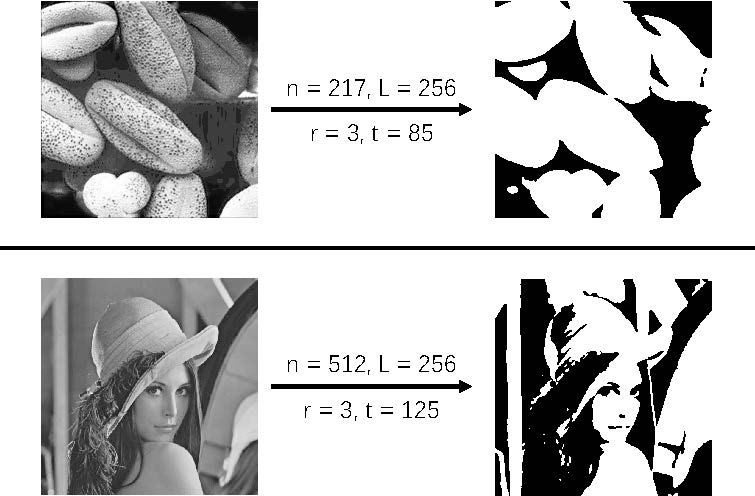
\includegraphics[width=0.95\textwidth]{image/22/2-p-1.jpg}
    % \caption{神经元 $v$ 变量随时间变化的曲线}
\end{figure}

现给定邻域参数 $r$ 和阈值 $t$,试统计输入灰度图像中有多少像素处于{\heiti{较暗区域}}。


\subsection*{输入格式}

输入共 $n + 1$ 行。

输入的第一行包含四个用空格分隔的正整数 $n$、$L$、$r$ 和 $t$,含义如前文所述。

第二到第 $n + 1$ 行输入矩阵 $A$。
第 $i + 2$($0 \le i < n$)行包含用空格分隔的 $n$ 个整数,依次为 $A_{i0}, A_{i1}, \cdots, A_{i(n-1)}$。


\subsection*{输出格式}

输出一个整数,表示输入灰度图像中处于较暗区域的像素总数。


